\documentclass{article}


% if you need to pass options to natbib, use, e.g.:
%     \PassOptionsToPackage{numbers, compress}{natbib}
% before loading neurips_2023


% ready for submission
\usepackage[preprint, nonatbib]{neurips_2023}
\usepackage{biblatex} %Imports biblatex package
\addbibresource{bosch.bib} %Import the bibliography file
\usepackage{graphicx}

% to compile a preprint version, e.g., for submission to arXiv, add add the
% [preprint] option:
%     \usepackage[preprint]{neurips_2023}


% to compile a camera-ready version, add the [final] option, e.g.:
%     \usepackage[final]{neurips_2023}


% to avoid loading the natbib package, add option nonatbib:
%    \usepackage[nonatbib]{neurips_2023}


\usepackage[utf8]{inputenc} % allow utf-8 input
\usepackage[T1]{fontenc}    % use 8-bit T1 fonts
\usepackage{hyperref}       % hyperlinks
\usepackage{url}            % simple URL typesetting
\usepackage{booktabs}       % professional-quality tables
\usepackage{amsfonts}       % blackboard math symbols
\usepackage{nicefrac}       % compact symbols for 1/2, etc.
\usepackage{microtype}      % microtypography
\usepackage{xcolor}         % colors


\title{Finding the causes of failure: Neuralwave 2024}


% The \author macro works with any number of authors. There are two commands
% used to separate the names and addresses of multiple authors: \And and \AND.
%
% Using \And between authors leaves it to LaTeX to determine where to break the
% lines. Using \AND forces a line break at that point. So, if LaTeX puts 3 of 4
% authors names on the first line, and the last on the second line, try using
% \AND instead of \And before the third author name.


\author{
	Mark Sobolev\\
	Faculty of Informatics\\
	Università della Svizzera Italiana\\
	Lugano, Switzerland \\
	\\
	% examples of more authors
	\And
	Marco Gabriel \\
	Faculty of Informatics \\
	Università della Svizzera Italiana\\
	Lugano, Switzerland \\
	% \\
	% \AND
	% Coauthor \\
	% Affiliation \\
	% Address \\
	% \texttt{email} \\
	% \And
	% Coauthor \\
	% Affiliation \\
	% Address \\
	% \texttt{email} \\
	% \And
	% Coauthor \\
	% Affiliation \\
	% Address \\
	% \texttt{email} \\
}


\begin{document}
	
	
	\maketitle
	

	\begin{abstract}
		We proposed a solution to a causal discovery in a multiple dataset context setting with a prior structural knowledge. Given the different measurements set, we produced a directed graph of causal influences and a ranking of influencing variables. In addition, we implemented a way to precisely constraint our causal model to reflect the changed mode. We developed a complex evaluation metric set for the unsupervised settings. Finally we designed a way to combine different approaches to causal discovery to produce the most reliable approach to generalised causal discovery setting. 
	\end{abstract}
	
	



	\section{Objective}
	
	We've been tackling a problem, where we were given several datasets with different latent context, for those we needed to provide the directed acyclic graph, which could be interpreted casually. Namely the datasets were structured as a set of columns, which were grouped in a several blocks, with an assumption of locality between elements of a block. We needed to discover various causal related structures about the given data:
	
	\begin{enumerate}
		\item The underlying causal graph
		\item The root causes of the observed change
		\item Visualisation of the graph, the root causes and their influence
	\end{enumerate}
	
	\subsection{Causal discovery}
	
	Causal discovery is a classic task, which also is extremely challenging. The causality discovery is used mainly in biology (Sachs, 2005) The task is to infer a Directed Acyclic Graph which minimizes a specific metric (which is trying to model causality) by observing the given data. The classic algorithms included using constrained-based approach to construct a graph (Glymour,2001: 5.4.2); the more novel ones usually vary in their assumptions (e.g. linearity and non-Gaussianity for DirectLiNGAM (Shimizu et al 2011)), but propose also more flexible ways to learn and evaluate the results (Zheng et al 2018). The complexity of the causal discovery relates to several facts: searching over the space of DAG is known to be NP-hard (Chickering 1996). 
	
	A recent major breakthrough in the field can be characterised by the introduction of a reformulation of a task to a continuous optimisation problem (Zheng, 2018); this introduced a family of new gradient-optimisational algorithms (Wang et al, 2021; Yu et al. 2019), however some skepticism is also present (Kaiser, 2021).
	
	\subsection{Evaluation of causal graph in unknown setting}
	
	As the task in a general setting should be solved without any ground truth given (except structural prior knowledge), one should come up with an algorithm for this. The task is not well researched, however there are some general strategies for doing such. First, you can divide your data to several sets, and try to evaluate your DAGs on the test data using Markov blanket (Pearl, 1986) , following (Wang, 2025). Second, a set of formal criterions for the graph evaluation can be suggested, such as generalizability (Yang, 2019), and graph falsifying metrics (Eulig, 2023). Both ways were computationally infeasible for us, so we've developed 4 intermediate strategies for the evaluation:
	
	\subsubsection{Peer dataset}
	
	The first way to evaluate the algorithms was by providing a helper dataset (i.e. the most popular nowadays IHDP (Shalit, 2017)), and evaluating datasets on that. As usually the causal discovery is done by using synthetic datasets (Cheng, 2022), it should be a good estimate for an implementation.
	
	\subsubsection{Distribution change evaluation}
	
	The second way was done by incorporating the fact that we had two different distributions for two datasets, thus the algorithm was to train the model on the first, prior dataset, and try to minimize the drop of causal estimation (with a helper regression algorithm e.g. XGBoost (Chen \& Guestrin, 2016)). 
	
	\subsubsection{Likelihood of the graph by the inner metrics}
	
	The third way is the comparison of the inner statistical metrics of different algorithms, e.g. p-values of the DirectLinGam \cite{lingam}. By this way the algorithms themselves report the quality of the output.
	
	\subsubsection{Predicting the data with the causal graph}
	
	This approach is based on training the regression and just comparing the output by the usual regression metrics, namely MSE or MAPE.
	
    \section{Approach} % Methodology, algorithms, and frameworks used.

    \subsection{Methodology}

    The process is divided into three stages. First, we do not have access to any ground-truth. In the second stage, we get access to the first 15 rows of the target adjacency-matrix. In the last stage, we get additional access to the lower diagonal adjacency-matrix. We use this ground-truth as prior knowledge in the following algorithms as well as to evaluate our results. To evaluate the performance, we calculate the Structural Hamming Distance (SHD) between the resulting adjacency matrix and the full ground truth.

    In every stage, we fit various algorithms to the given data and compared their results. We outline these algorithms and the used frameworks in the following sections.

    \subsection{Algorithms}
    
    \subsubsection{Causal discovery with Ordering-based Reinforcement
    Learning (CORL)}
    CORL\cite{CORL} uses a Reinforcement Learning (RL) approach and is implemented in the gCastle Framework. 

    \subsection{DAG\_GNN}
    In DAG-GNN \cite{DAGGNN}, the problem is formulated as a continuous optimization problem and solved using a generative model. It is impllemented in gCastle. 

    \subsubsection{LiNGAM}
    LiNGAM estimates structural equation models or linear causal Bayesian networks, assuming the data is non-Gaussian.
    First, to apply DirectLiNGAM\cite{lingam}, we merge the datasets while introducing a new feature to differentiate the origins. 
    Secondly, we use MultiGroupDirectLiNGAM: \cite{multilingam} on the separate datasets.
    Additionally, we try Independent component analysis (ICA-LiNGAM)\cite{ICALINGAM} which assumes the observed variables to be linear functions of mutually independent and non-Gaussian disturbance variables.

    \subsubsection{Fast Causal Inference (FCI)}
    The FCI algorithm \cite{FCI} works under both latent variables and selection bias. We use its implementation in causal-learn \cite{Causallearn}.

	
	\subsubsection{VAR-LINGRAM}
	
	Var-Lingram (Shimizu, 2006)	 is a time series extension for a Lingram model. The linearity of a data-generating process was an important contribution, due to the similarity with our structural constraints.    


    \subsubsection{Peter-Clark (PC)}
    PC \cite{PC} is a general purpose algorithms for causal discovery which works by first identifying the undirected causal graph, and then directing the edges. It is also implemented in causal-learn.
    
    \subsubsection{Structural Agnostic Model (SAM)}
    We use the SAM\cite{SAM} implementation of the CausalDiscoveryToolbox (CDT). SAM implements an adversarial game in which separate models generate each variable based on the real observations from all other variables, on the hypothesis, that the target variable depends on those. A discriminator then attempts to distinguish between real and generated samples. Finally, a sparsity penalty forces each generator to consider only a small subset of the variables, yielding a sparse causal graph. SAM allows to alleviate the commonly made condition, that there is no hidden common cause to any pair of observed variables.
    It is shown to be orders of magnitudes slower than LiNGAM for example, but also significantly better.

    \subsubsection{LLM: o1-preview from OpenAI}
    We prompt the o1-preview LLM from OpenAI to respond with the nodes causing the increased value, given the datasets.
    
    \subsection{Frameworks}
    \subsubsection{DoWhy}
    The key feature of DoWhy \cite{DoWhy} \cite{sharma2020dowhyendtoendlibrarycausal} is that it provides algorithms for the refutation and falsification of causal graphs.
    
    
    \subsubsection{CausalDiscoveryToolbox (CDT)}
    The CausalDiscoveryToolbox supports causal inference in graphs and in pairwise settings. It implements several algorithms, including the PC, LiNGAM, and SAM algorithms.
    https://github.com/FenTechSolutions/CausalDiscoveryToolbox 
    \cite{CDT}
    
    \subsubsection{gCastle}
    GCastle is a causal structure learning toolchain containing various functionalities related to causal learning such as the PC and LiNGAM algorithms. 
    \cite{zhang2021gcastlepythontoolboxcausal}
    
    \section{Results} % Key findings, metrics, or visualizations.

    \subsection{Causal Graph}

    Comparing the various algorithms to discover causal graphs, we found LiNGAM to produce good quality graphs while being significantly faster than many others. DUe to these findings, we chose it for our final implementation. An excerpt of the comparisons we did can be seen in Table \ref{comparisonSHD}.

    The final resulting graph is shown in Fig \ref{fig:wholegraph}.
    
    \begin{table}
		\caption{Comparison of different Algorithms}
		\label{comparisonSHD}
		\centering
		\begin{tabular}{lr}
			\toprule
			\multicolumn{2}{c}{Part}                   \\
			\cmidrule(r){1-2}
			Name     & SHD Distance to ground truth (lower is better)  \\
			\midrule
			CORL  & 493       \\
			DAG\_GNN & 543    \\
			PC & 523     \\
            FCI  & 523 \\
			\bottomrule
		\end{tabular}
	\end{table}

     \begin{figure}
         \centering
         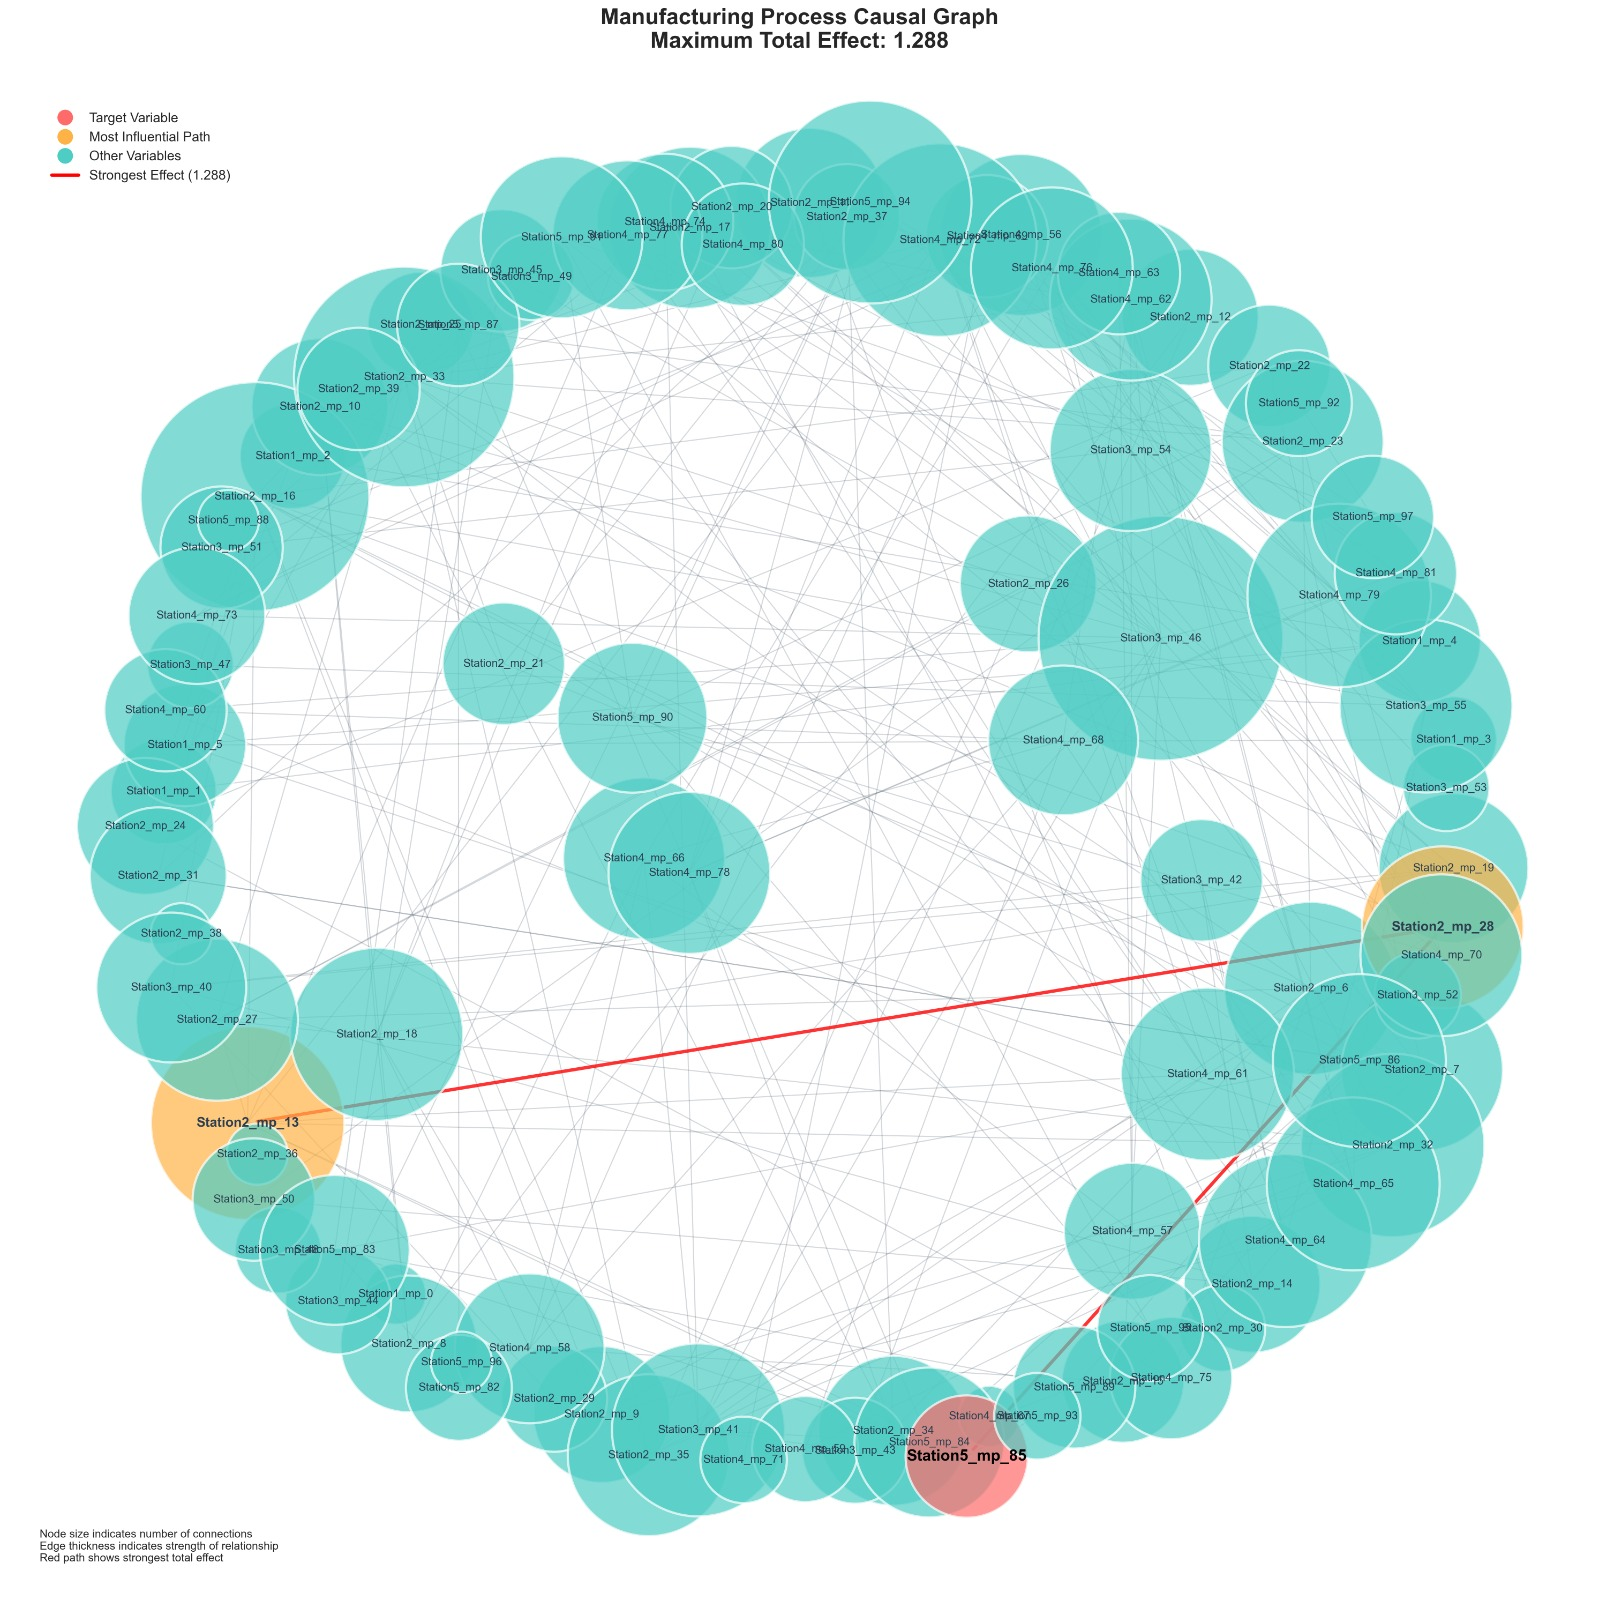
\includegraphics[width=0.75\linewidth]{whole_graph_result.jpeg}
         \caption{The entire causal graph}
         \label{fig:wholegraph}
     \end{figure}
    
    \subsection{Root Cause}
    
    The sub-graph showing the root cause is visualised in Fig. \ref{fig:subgraph}.
    \begin{figure}
        \centering
        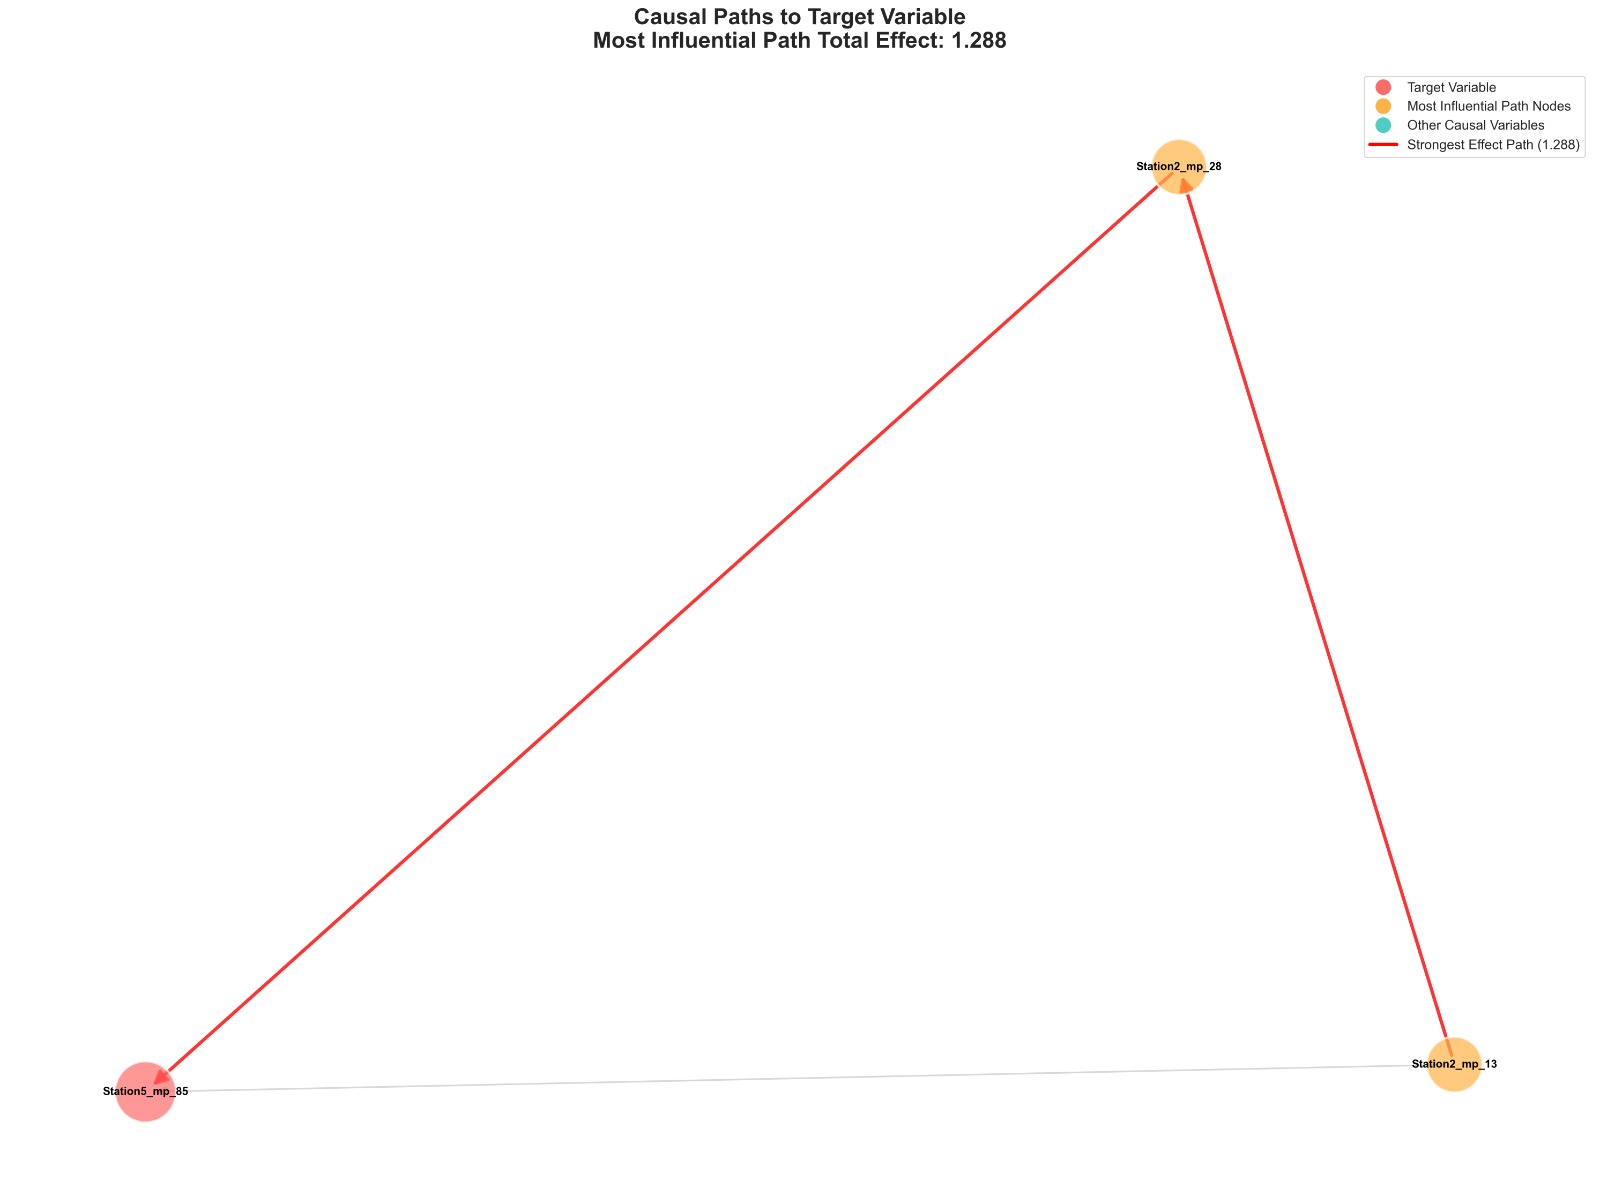
\includegraphics[width=0.75\linewidth]{subgraph_result.jpeg}
        \caption{The sub-graph showing the root cause, from Station2\_mp\_13 to Station2\_mp\_28 to Station5\_mp\_85.}
        \label{fig:subgraph}
    \end{figure}
    
    \subsection{Visualisation}

    To visualize the root cause, we mainly show all nodes that feed into the target node. This is achieved by inverting the found adjacency matrix and starting from the target node, visit all its descendants recursively. Thus, we get the sub-graph of all nodes influencing the target node. 

    Further, we identify the most influential path according to its total effect on the target node, as seen in Fig. \ref{fig:subgraph}.
    
    
    \section{Challenges} % Difficulties encountered and solutions.
    The most challenging issue throughout the process was to evaluate possible solutions without knowing the ground truth or just having partial ground truth.


	
	
	
	
	
	
	
	
	
	\printbibliography %Prints bibliography
	%%%%%%%%%%%%%%%%%%%%%%%%%%%%%%%%%%%%%%%%%%%%%%%%%%%%%%%%%%%%
	
	
\end{document}